\chapter{Funktionale Anforderungen / Use Case}

	\section{Use Case Diagramm}    
    \begin{figure}[h]
    	\centering
    	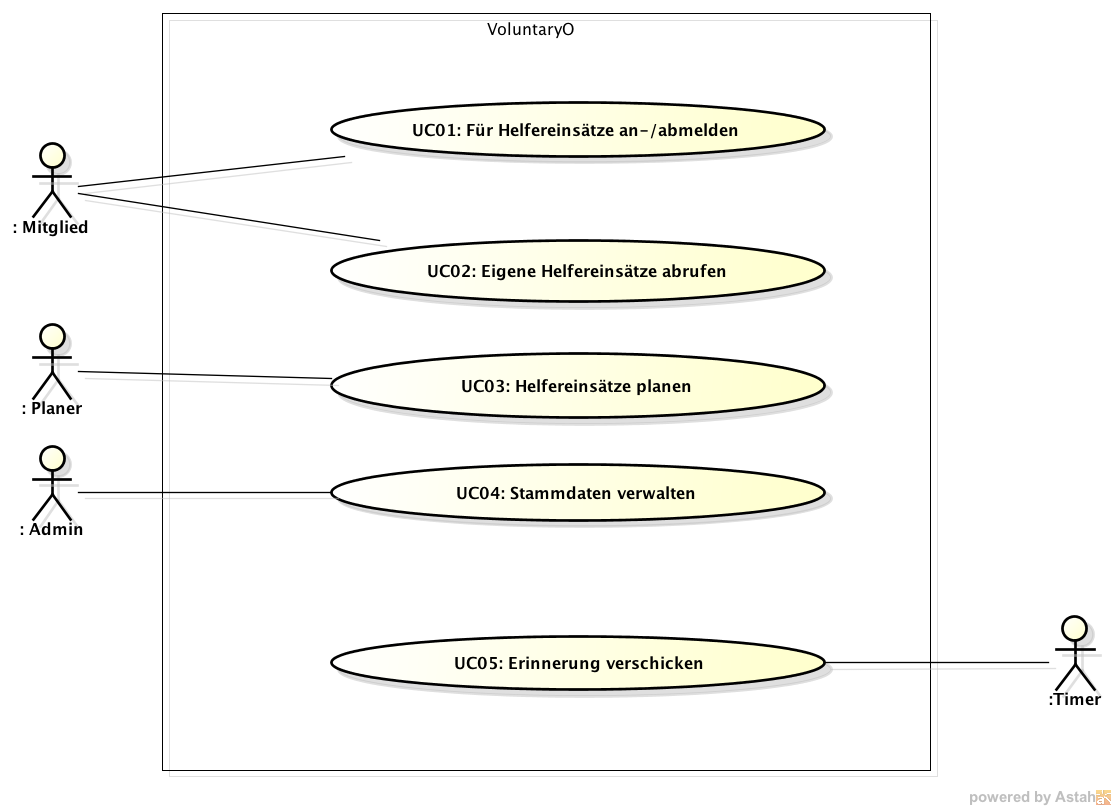
\includegraphics[width=0.9\textwidth]{content/anforderungsspezifikation/images/usecase_diagram.png}
    	\caption{Use Case Diagramm}
	\end{figure}
	
	\section{Use Cases brief Format}
    \begin{table}[H]
        \tablestyle
        \tablealtcolored
        \begin{tabularx}{\textwidth}{l X l}
            \tablebody
            \textbf{Use Case Name} &
                UC01: Benutzer anmelden/abmelden
                \tabularnewline
            \textbf{Ref. Primäre Funktionen} &
                \textit{-}
                \tabularnewline
            \textbf{Zusammenfassung} &
                Benutzer (User, Planer, Admin ) können sich authentifizieren. Danach erhalten sie Zugang zur Applikation, entsprechend ihren Berechtigungen (Autorisierung).
                \tabularnewline
            \textbf{Main Success Szenario} &
                Benutzer gibt seinen Namen und das Passwort an. Das System überprüft die Richtigkeit der Angaben und stattet den Benutzer mit seinen Rechten aus. 
                \tabularnewline
                \textbf{Actors} &
                User, Planer, Admin
                \tabularnewline
                \textbf{Extends} &
                
                \tabularnewline
            \tableend
        \end{tabularx}
    \end{table}
    
    \begin{table}[H]
        \tablestyle
        \tablealtcolored
        \begin{tabularx}{\textwidth}{l X l}
            \tablebody
            \textbf{Use Case Name} &
                UC02: Für Helfereinsatz eintragen
                \tabularnewline
            \textbf{Ref. Primäre Funktionen} &
                \textit{F08}, \textit{F09}
                \tabularnewline
            \textbf{Zusammenfassung} &
                Für jedes Event gibt es vorgegeben Helfereinsätze ( = „Tätigkeiten“). Benutzer können sich für diese Tätigkeiten eintragen und auch wieder abmelden.
                \tabularnewline
            \textbf{Main Success Szenario} &
                Benutzer wählt Helfereinsatz aus und meldet sich dafür an oder ab. System überprüft Sperrfrist und lässt An- bzw. Abmeldung zu, falls Sperrfrist nicht überschritten wurde.
                \tabularnewline
                \textbf{Actors} &
                User
                \tabularnewline
                \textbf{Extends} &
                
                \tabularnewline
            \tableend
        \end{tabularx}
    \end{table}
    
    \begin{table}[H]
        \tablestyle
        \tablealtcolored
        \begin{tabularx}{\textwidth}{l X l}
            \tablebody
            \textbf{Use Case Name} &
                UC03: Helfereinsätze anzeigen 
                \tabularnewline
            \textbf{Ref. Primäre Funktionen} &
                \textit{F10}
                \tabularnewline
            \textbf{Zusammenfassung} &
                Benutzer kann sich seine Helfereinsätze anzeigen lassen.
                \tabularnewline
            \textbf{Main Success Szenario} &
                Benutzer fragt Helfereinsätze ab. System liefert alle Helfereinsätze, für die der Benutzer angemeldet ist.
                \tabularnewline
                \textbf{Actors} &
                User
                \tabularnewline
                \textbf{Extends} &
                
                \tabularnewline
            \tableend
        \end{tabularx}
    \end{table}
    
    \begin{table}[H]
        \tablestyle
        \tablealtcolored
        \begin{tabularx}{\textwidth}{l X l}
            \tablebody
            \textbf{Use Case Name} &
                UC04: Helfereinsatz Details anzeigen 
                \tabularnewline
            \textbf{Ref. Primäre Funktionen} &
                \textit{F08}
                \tabularnewline
            \textbf{Zusammenfassung} &
                -
                \tabularnewline
            \textbf{Main Success Szenario} &
                Benutzer wählt Helfereinsatz aus und fragt Details ab. System liefert Detailinformationen (Beschreibung, Uhrzeit, Ort, min. Personen, max. Personen, angemeldete Personen, Vorraussetzungen).
                \tabularnewline
                \textbf{Actors} &
                User
                \tabularnewline
                \textbf{Extends} &
                
                \tabularnewline
            \tableend
        \end{tabularx}
    \end{table}
    
    \begin{table}[H]
        \tablestyle
        \tablealtcolored
        \begin{tabularx}{\textwidth}{l X l}
            \tablebody
            \textbf{Use Case Name} &
                UC05: Export der Termine (optional) 
                \tabularnewline
            \textbf{Ref. Primäre Funktionen} &
                \textit{F31}
                \tabularnewline
            \textbf{Zusammenfassung} &
                Helfereinsätze als Termine exportieren.
                \tabularnewline
            \textbf{Main Success Szenario} &
                Der Benutzer exportiert die Übersicht seiner Helfereinsätze in ein Kalenderformat (bspw. iCal).
                \tabularnewline
                \textbf{Actors} &
                User
                \tabularnewline
                \textbf{Extends} &
                
                \tabularnewline
            \tableend
        \end{tabularx}
    \end{table}
    
    \begin{table}[H]
        \tablestyle
        \tablealtcolored
        \begin{tabularx}{\textwidth}{l X l}
            \tablebody
            \textbf{Use Case Name} &
                UC06: Events verwalten CRUD 
                \tabularnewline
            \textbf{Ref. Primäre Funktionen} &
                \textit{F04}
                \tabularnewline
            \textbf{Zusammenfassung} &
                Der Planer ist zuständig für die Verwaltung von Events. Ein Event ist die Grundlage für die einzelnen Helfereinsätze. Neue Events sollen hinzugefügt werden können und diese auch bearbeitet oder entfernt werden können.
                \tabularnewline
            \textbf{Main Success Szenario} &
                Der Planer ist in der Lage alle Events zu verwalten
                \tabularnewline
                \textbf{Actors} &
                Planer
                \tabularnewline
                \textbf{Extends} &
                
                \tabularnewline
            \tableend
        \end{tabularx}
    \end{table}
    
    \begin{table}[H]
        \tablestyle
        \tablealtcolored
        \begin{tabularx}{\textwidth}{l X l}
            \tablebody
            \textbf{Use Case Name} &
                UC07: Events importieren
                \tabularnewline
            \textbf{Ref. Primäre Funktionen} &
                \textit{F03}
                \tabularnewline
            \textbf{Zusammenfassung} &
                Falls in einem externen System neue Events vorhanden sind, soll der Planer die Möglichkeit haben diese in das System zu importieren. Die Events werden dann über einen Webservice geladen.
                \tabularnewline
            \textbf{Main Success Szenario} &
                Die Events werden in das System importiert. Fehlerhafte Events sollen angezeigt werden. Die Events sollen innerhalb des Systems verwaltbar sein.
                \tabularnewline
                \textbf{Actors} &
                Planer
                \tabularnewline
                \textbf{Extends} &
                Events verwalten
                \tabularnewline
            \tableend
        \end{tabularx}
    \end{table}
    
    \begin{table}[H]
        \tablestyle
        \tablealtcolored
        \begin{tabularx}{\textwidth}{l X l}
            \tablebody
            \textbf{Use Case Name} &
                UC08: Einsätze für Event verwalten CRUD
                \tabularnewline
            \textbf{Ref. Primäre Funktionen} &
                \textit{F01}, \textit{F02}
                \tabularnewline
            \textbf{Zusammenfassung} &
                Jeder Event hat mehrere Helfereinsätze. Diese müssen vom Planer verwaltet werden.
                \tabularnewline
            \textbf{Main Success Szenario} &
                Der Planer kann verschiedene Helfereinsätze hinzufügen und diese ändern.
                \tabularnewline
                \textbf{Actors} &
                Planer
                \tabularnewline
                \textbf{Extends} &
                
                \tabularnewline
            \tableend
        \end{tabularx}
    \end{table}
    
    \begin{table}[H]
        \tablestyle
        \tablealtcolored
        \begin{tabularx}{\textwidth}{l X l}
            \tablebody
            \textbf{Use Case Name} &
                UC09: Benutzer verwalten CRUD
                \tabularnewline
            \textbf{Ref. Primäre Funktionen} &
                \textit{F06}
                \tabularnewline
            \textbf{Zusammenfassung} &
                Die verschiedenen Benutzer sollen vom Admin verwaltet werden. Neue Benutzer sollen hinzugefügt werden können oder Passwörter geändert werden.
                \tabularnewline
            \textbf{Main Success Szenario} &
                Der Admin kann einen neuen Benutzer hinzufügen und dessen Passwort und Rolle setzen.
                \tabularnewline
                \textbf{Actors} &
                Admin
                \tabularnewline
                \textbf{Extends} &
                
                \tabularnewline
            \tableend
        \end{tabularx}
    \end{table}
    
    \begin{table}[H]
        \tablestyle
        \tablealtcolored
        \begin{tabularx}{\textwidth}{l X l}
            \tablebody
            \textbf{Use Case Name} &
                UC10: Benutzer importieren
                \tabularnewline
            \textbf{Ref. Primäre Funktionen} &
                \textit{F05}
                \tabularnewline
            \textbf{Zusammenfassung} &
                Die Benutzer sollen neben der manuellen Erstellung auch aus einem externen System importiert werden können. Diese Benutzer sollen über einen Webservice abgerufen werden können.
                \tabularnewline
            \textbf{Main Success Szenario} &
                Die neuen Benutzer werden in das System importiert. Fehlerhafte Benutzer sollen angezeigt werden. Diese Benutzer sollen danach verwaltbar sein.
                \tabularnewline
                \textbf{Actors} &
                Admin
                \tabularnewline
                \textbf{Extends} &
                Benutzer verwalten
                \tabularnewline
            \tableend
        \end{tabularx}
    \end{table}
    
    \begin{table}[H]
        \tablestyle
        \tablealtcolored
        \begin{tabularx}{\textwidth}{l X l}
            \tablebody
            \textbf{Use Case Name} &
                UC11: Erinnerungen verschicken
                \tabularnewline
            \textbf{Ref. Primäre Funktionen} &
                \textit{F11}
                \tabularnewline
            \textbf{Zusammenfassung} &
                Für jeden Event sollen an vordefinierten Zeitpunkten Erinnerungen an alle angemeldeten Benutzer versendet werden können.
                \tabularnewline
            \textbf{Main Success Szenario} &
                Es wird automatisch eine Erinnerung an jeden im Event angemeldeten Benutzer gesendet.
                \tabularnewline
                \textbf{Actors} &
                Timer
                \tabularnewline
                \textbf{Extends} &
               	
                \tabularnewline
            \tableend
        \end{tabularx}
    \end{table}
